% Provenance (never printed): see sources/outline_sources.md (Year 2: oceanic islands; growth,
% flank collapse and erosion of volcanic islands; reefs and atolls; subsidence). Hawaiian
% stages, slides, subsidence and drowned reefs after Clague and Sherrod (2014, USGS PP 1801
% ch. 3) and Denlinger and Morgan (2014, ch. 4); the Nuuanu slide after the ODP Leg 200 report;
% the Enewetak holes after Ladd and Schlanger (1960, USGS PP 260-Y); Kure after the NOAA
% monument pages; the depth--age law from the Book 2 and Book 3 rows. Curves and the invented
% Petrel island from figdata/bachelor-2/islands.py; exercise and problem values in the Book 4
% scratch calculator calc/ch17.py.
\chapter{Oceaaneilanden}\label{ch:b2:oceanic-islands}

In 1952 gingen op twee eilanden van het \omterm{def:b2:oceanic-islands:reefs}{atol} Enewetak in de westelijke Stille Oceaan (toen Eniwetok gespeld) twee
boorgaten door koraalgesteente naar meer dan \qty{1.2}{km} diepte. Op Parry Island bracht de boor
boorgruis van vers basalt boven op een diepte van 4158 voet, \qty{1267}{m}, en daarna een kern van
olivijnbasalt. Daarboven lag kalksteen uit het Eoceen, vol rifkoralen van een soort die niet
dieper groeit dan ongeveer \qty{46}{m}. Een koraalrif was ooit vlak bij zeeniveau gegroeid op de schouders van een vulkaan,
en de vulkaan was meer dan een kilometer gezonken terwijl het rif er bovenop bleef
groeien. Dit hoofdstuk volgt een \omterm{def:b2:oceanic-islands:stages}{oceaaneiland} door zijn hele leven: hoe het groeit, hoe zijn flanken
in zee vallen, waarom het zinkt en hoe een ring van koraal het kan overleven.
% ledger: ls60:enewetak, ics4:eocene

\begin{recall}
\textbf{Uit Boek~3}: hotspot, mantelpluim, hotspotspoor en zijn ouderdomsprogressie,
de Hawaïaans–Emperor-keten en de Hawaïaanse zwelling; de diepte--ouderdomswet van de oceaanbodem; riffen,
hun vormen als \omterm{def:b2:oceanic-islands:reefs}{kustrif}, \omterm{def:b2:oceanic-islands:reefs}{barrièrerif} en \omterm{def:b2:oceanic-islands:reefs}{atol} zoals Darwin ze beschreef, en de regel ``bijhouden of
verdrinken''; eustasie en de zeespiegel van het laatste glaciale maximum, ongeveer \qty{120}{m} lager dan
vandaag. \textbf{Uit de schoolboeken}: de schildvulkaan; het abrasieplatform.
\textbf{Uit \cref{ch:b2:magmatic-series}}: de tholeïtische en de \omterm{def:b2:magmatic-series:series}{alkalische reeks}.
\end{recall}

\section{De groei van een vulkanisch eiland}\label{sec:b2:oceanic-islands:growth}

De Hawaï-eilanden zijn het jongste uiteinde van de keten die Boek~3 over de
noordelijke Stille Oceaan volgde. De hoofdeilanden tellen 19 bekende schildvulkanen: 15 staan boven de zee,
3 liggen onder water, en één, pas geboren, is nog onderzees. Terwijl de Pacifische plaat ze naar het
noordwesten draagt, wordt elk boven de hotspot geboren, groeit, sterft terwijl hij wegdrijft, en zinkt. Dat leven is
regelmatig genoeg om in stadia te worden opgedeeld.
% ledger: cs14:volcanoes

\begin{definition}[Oceaaneiland; groeistadia]\label{def:b2:oceanic-islands:stages}
Een \emph{oceaaneiland}\index{oceaaneiland} is een vulkanisch eiland dat oprijst uit de
oceaanbodem en gebouwd is op oceanische lithosfeer. Een eiland van een hotspotketen doorloopt vier eruptieve
stadia: een \emph{preschildstadium} van kleine erupties van alkalische lava op de zeebodem; het
\emph{schildstadium}\index{schildstadium}, waarin tholeïtische lava het grootste deel van de vulkaan opbouwt
terwijl die boven de hotspot ligt; een \emph{postschildstadium} van minder talrijke, meer alkalische erupties,
die het schild afdekken; en, na een pauze, een \emph{verjongd stadium} van zeldzame, kleine alkalische
erupties. Daarna nemen erosie en wegzinken het over.
\end{definition}
% ledger: usgs14:hawaii-stages, cs14:rejuvenated

De stadia volgen de toevoer van warmte. Loihi, de jongste vulkaan, ligt \qty{54}{km} ten zuiden van de
top van de Kilauea; zijn top ligt nog \qty{975}{m} onder de zee, maar al \qty{2.5}{km} boven de
zeebodem eromheen, en zijn oudste lava's zijn alkalisch. In het \omterm{def:b2:oceanic-islands:stages}{schildstadium} ligt de vulkaan boven
de hotspot en wordt hij het snelst gevoed. Elke Hawaïaanse vulkaan stoot in dit stadium naar schatting 80 tot
\qty{95}{\percent} van zijn uiteindelijke volume uit, grotendeels binnen zijn eerste 1 tot \qty{2}{Myr}.
Laat in het stadium daalt de eruptiesnelheid met een factor tien. De ondiepe magmareservoirs, 1
tot \qty{7}{km} diep, kunnen niet langer in leven worden gehouden, al blijven kleinere op 20 tot \qty{30}{km}
bestaan. De lava wordt weer alkalisch, omdat een lagere smeltgraad haar dat karakter geeft, zoals
\cref{ch:b2:magmatic-series} liet zien. Het verjongde stadium komt na een pauze van minder dan 0.5
tot \qty{2.0}{Myr}. Het kan één of twee episoden omvatten, of heel lang duren: op Niihau duurde het van 2.2 tot
\qty{0.4}{Ma}, en op Kauai gaat het door sinds \qty{3.5}{Ma}.
% ledger: cs14:loihi, usgs14:hawaii-stages, cs14:rejuvenated

De volumes zijn enorm. Het volume van de Mauna Loa wordt geschat op ongeveer \qty{74000}{km^3}. Wanneer de grens met de Kilauea opnieuw wordt getrokken zodat de Kilauea slechts ongeveer
\qty{10000}{km^3} houdt, stijgt het aandeel van de Mauna Loa tot \qty{95600}{km^3}. De jonge Loihi bevat
\qty{1700}{km^3}. De hele keten komt sinds \qty{81}{Ma} op ongeveer
\qty{2e6}{km^3}; een eruptiesnelheid geïntegreerd over die geschiedenis, \qty{0.07}{km^3} per jaar, zou bijna drie keer zoveel opleveren. De last is zwaar genoeg om de
plaat te buigen: de oceaankorst onder de eilanden wordt tot \qty{5}{km} omlaaggedrukt, langs een
trog die de Hawaïaanse Gracht heet, en een lage bolling, de Hawaïaanse Welving, rijst enkele honderden
kilometers verderop. Hoe een plaat onder een last buigt, komt in Boek~5 aan bod. Hier
is de gracht van belang omdat een groot deel van het puin van de eilanden er terechtkomt.
% ledger: cs14:volumes, cs14:loihi, cs14:moat

\begin{omfigure}
\centering
\begin{tikzpicture}[x=0.95cm, y=0.95cm, font=\footnotesize]
% schematic, not to scale (vertical exaggeration about 10). Sea level y = 0; sea floor
% y = -1.6 - 0.0625 (16 - x), deepening with the age of the plate to the left.
\fill[omSea!45] (0,0) -- (16,0) -- (16,-1.6) -- (0,-2.6) -- cycle;
\fill[black!18] (0,-2.6) -- (16,-1.6) -- (16,-3.1) -- (0,-3.1) -- cycle;
\draw[black!60] (0,-2.6) -- (16,-1.6);
\draw[omSea!60!black] (0,0) -- (16,0);
\node[anchor=south, font=\scriptsize] at (8.7,0) {zeeniveau};
% (a) shield stage over the hotspot
\fill[lith basalt, draw=black!70] (12.6,-1.8125) -- (13.9,0.75) -- (14.3,0.9) -- (14.7,0.75) -- (16,-1.6) -- cycle;
% (b) eroded island with a fringing reef (valleys notched in the summit)
\fill[lith basalt, draw=black!70] (9.2,-2.025) -- (10.1,0.15) -- (10.3,0.35) -- (10.45,0.2) -- (10.6,0.45) -- (10.8,0.25) -- (11.0,0.3) -- (11.2,0.1) -- (12.0,-1.85) -- cycle;
\fill[lith reef limestone, draw=black!70] (10.038,0) -- (9.976,-0.15) -- (9.80,0) -- cycle;
\fill[lith reef limestone, draw=black!70] (11.241,0) -- (11.303,-0.15) -- (11.46,0) -- cycle;
% (c) barrier reef around a smaller island, a lagoon between
\fill[lith basalt, draw=black!70] (5.8,-2.2375) -- (7.0,0.2) -- (8.2,-2.0875) -- cycle;
\fill[lith reef limestone, draw=black!70] (6.384,-1.05) -- (6.42,0) -- (6.60,0) -- (6.62,-0.45) -- (6.680,-0.45) -- cycle;
\fill[lith reef limestone, draw=black!70] (7.656,-1.05) -- (7.62,0) -- (7.44,0) -- (7.42,-0.45) -- (7.341,-0.45) -- cycle;
% (d) atoll: volcano bevelled and drowned, reef cap with a lagoon
\fill[lith basalt, draw=black!70] (2.7,-2.43125) -- (3.6,-0.55) -- (4.0,-0.55) -- (4.9,-2.29375) -- cycle;
\fill[lith reef limestone, draw=black!70] (3.4325,-0.9) -- (3.47,0) -- (4.14,0) -- (4.1806,-0.9) -- (4.0,-0.55) -- (3.6,-0.55) -- cycle;
\fill[omSea!45] (3.62,-0.15) rectangle (3.99,0);
% (e) guyot: flat top with a drowned reef cap, beyond the Darwin point
\fill[lith basalt, draw=black!70] (0.2,-2.5875) -- (0.9,-0.95) -- (1.7,-0.95) -- (2.4,-2.475) -- cycle;
\fill[lith reef limestone, draw=black!70] (0.9,-0.95) -- (0.96,-0.75) -- (1.64,-0.75) -- (1.7,-0.95) -- cycle;
% Darwin point
\draw[black!70, dashed] (2.55,0.55) -- (2.55,-2.5);
\node[anchor=south, font=\scriptsize] at (2.55,0.55) {Darwinpunt};
% hotspot and plate motion
\draw[omThm, line width=1.4pt, -{Stealth[length=2.5mm]}] (14.3,-3.9) -- (14.3,-3.15);
\node[anchor=west, font=\scriptsize, text=omThm] at (14.4,-3.7) {hotspot};
\draw[black, line width=0.8pt, -{Stealth[length=2.5mm]}] (9.5,-2.85) -- (6.5,-2.85);
\node[anchor=west, font=\scriptsize] at (9.6,-2.85) {plaatbeweging};
\node[anchor=west, font=\scriptsize] at (0.1,-2.9) {oceanische lithosfeer};
% stadialabels
\node[align=center, font=\scriptsize] at (14.3,1.45) {(a) schildstadium};
\node[align=center, font=\scriptsize] at (10.6,1.3) {(b) geërodeerd eiland,\\ kustrif};
\node[align=center, font=\scriptsize] at (7.0,1.45) {(c) barrièrerif};
\node[align=center, font=\scriptsize] at (3.8,1.45) {(d) atol};
\node[align=center, font=\scriptsize] at (1.3,1.45) {(e) guyot};
\draw[black!60, -{Stealth[length=2mm]}] (13.6,-3.7) -- (0,-3.7);
\node[anchor=south, font=\scriptsize, fill=white, inner sep=1pt] at (7,-3.7) {oudere vulkanen, oudere en diepere plaat};
\end{tikzpicture}
\par\smallskip{\small Het leven van een \omterm{def:b2:oceanic-islands:stages}{oceaaneiland}, gelezen langs een hotspotketen (schematisch, niet op
schaal, verticale schaal sterk overdreven). De plaat voert elke vulkaan weg van de hotspot
(rechts) en de vulkaan zinkt mee, terwijl erosie hem afslijt. (a)~Een schildvulkaan groeit boven
de hotspot. (b)~Uitgedoofd en geërodeerd wordt hij door riffen omzoomd. (c)~Verder gezonken is hij omgeven
door een \omterm{def:b2:oceanic-islands:reefs}{barrièrerif} met een lagune erachter. (d)~Zijn top is onder de zee verdwenen, en een rifkap met
een centrale lagune, een \omterm{def:b2:oceanic-islands:reefs}{atol}, groeit er bovenop. (e)~Meegevoerd naar water dat te koel is voor het rif om
bij te houden, verdrinkt het \omterm{def:b2:oceanic-islands:reefs}{atol} en zinkt het als een \omterm{def:b2:oceanic-islands:seamount}{guyot} met een platte top.}
\end{omfigure}
% ledger: cs14:volcanoes, cs14:erase, cs14:darwin-point, pmnm:geology

\section{Flankinstorting}\label{sec:b2:oceanic-islands:collapse}

Een vulkaan van enkele kilometers hoog, gebouwd uit losse lavastromen en puin, staande op hellingen die
afdalen in de gracht, is niet stabiel. In 1975 verplaatste de aardbeving van Kalapana, met magnitude 7.7,
de zuidflank van de Kilauea in één keer tot \qty{10}{m} zeewaarts en veroorzaakte een tsunami. In
1868 ging een andere flankbeweging gepaard met een aardbeving van magnitude 7.9 en een tsunami die 46
mensen doodde. Seismische profielen onder deze flanken tonen een diepe reflector. Die wordt gelezen als een
\omterm{def:b2:alpine-orogen:decollement}{décollement} langs de top van de oude oceaankorst, waarop de hele flank glijdt. Meestal kruipt de
flank; soms bezwijkt hij.
% ledger: dm14:flank

\begin{definition}[Flankinstorting; puinlawine; slump]\label{def:b2:oceanic-islands:collapse}
Een \emph{flankinstorting}\index{flankinstorting} is het bezwijken van een groot deel van de flank van een
vulkaan, dat onder zijn eigen gewicht wegglijdt. Wanneer de bewegende massa uiteenvalt en snel
uitloopt, als een stroom van blokken en puin die ver voorbij de voet van de vulkaan kan reizen, is het een
\emph{puinlawine}\index{puinlawine}. Wanneer ze langzaam beweegt, als grote blokken die roteren
op breuken die in een diep \omterm{def:b2:alpine-orogen:decollement}{décollement} wortelen, en dicht bij de vulkaan blijft, is het een \emph{slump}.
\end{definition}

Het bewijs ligt onder de zee. Eind jaren 1980 toonde het karteren van de wateren rond de
Hawaï-eilanden met zijwaarts kijkende sonar puin dat over de diepe zeebodem verspreid lag, honderden kilometers van
de eilanden, en slumps uit grote, in segmenten opgedeelde blokken. Rond de hoofdeilanden werden zeventien grote afschuivingen
herkend, gevormd in de laatste \qty{5}{Myr}. Zeventig zijn er nu bekend langs de
Hawaïaanse Rug tussen het eiland Hawaï en Midway, gevormd over \qty{30}{Myr}. Dat is ten
minste één afschuiving per \qty{300}{kyr} rond de hoofdeilanden. Deze aantallen zijn minima, omdat een
jongere vulkaan het litteken en het puin van een oudere kan begraven: de topcaldera en een riftzone
van Niihau ontbreken, en er is geen afzetting voor gevonden. De reusachtige afschuivingen lijken het waarschijnlijkst terwijl de
vulkaan het snelst groeit, van het late preschild- tot het vroege postschildstadium, maar ze gaan
lang daarna door.
% ledger: cs14:slides, dm14:flank

De grootste is de Nuuanu-afschuiving, die de noordoostflank van de Koolau-vulkaan
op Oahu wegrukte. Het is een \omterm{def:b2:oceanic-islands:collapse}{puinlawine} die over \qty{23000}{km^2} is uitgespreid en zich meer dan
\qty{200}{km} van het eiland uitstrekt. Tot haar blokken behoort de \omterm{def:b2:oceanic-islands:seamount}{Tuscaloosa-zeeberg}, ongeveer \qty{30}{km} lang,
\qty{17}{km} breed en minstens \qty{2}{km} hoog. De lawine stak de diepe gracht over en klom
meer dan \qty{100}{km} de helling van de Hawaïaanse Welving op. Haar ouderdom wordt geschat op 2.1 tot
\qty{1.8}{Ma}, tegen het einde van het leven van de Koolau of daarna; zijn oppervlaktelava's zijn 1.8 tot
\qty{2.6}{Ma} oud. Uit hoeveel instortingen ze bestond, en hoe dik ze ver van het eiland is,
zijn nog open vragen.
% ledger: odp200:nuuanu

\begin{omfigure}
\centering
\begin{tikzpicture}[x=0.95cm, y=0.95cm, font=\footnotesize]
% schematic section from the summit of an island (left) across the moat to the arch (right);
% not to scale. Sea level y = 0; top of the old oceanic crust, bent down under the island.
\fill[omSea!45] (0,0) -- (15,0) -- (15,-2.2) -- (13.5,-2.12) -- (11,-2.05) -- (8.5,-2.35) -- (6.5,-2.75) -- (5.6,-2.82) -- (4.0,-1.4) -- (2.5,0) -- cycle;
\fill[black!18] (0,-3.05) -- (5.6,-2.82) -- (6.5,-2.75) -- (8.5,-2.35) -- (11,-2.05) -- (13.5,-2.12) -- (15,-2.2) -- (15,-3.6) -- (0,-3.6) -- cycle;
\draw[black!70] (0,-3.05) -- (5.6,-2.82) -- (6.5,-2.75) -- (8.5,-2.35) -- (11,-2.05) -- (13.5,-2.12) -- (15,-2.2);
\draw[omSea!60!black] (0,0) -- (15,0);
\node[anchor=south east, font=\scriptsize] at (15,0) {zeeniveau};
% the volcano: present flank (after collapse) and the lost flank (dashed)
\fill[lith basalt, draw=black!70] (0,1.15) -- (0.8,1.05) -- (1.25,0.95) -- (1.45,0.45) -- (1.75,0.1) -- (2.6,-0.75) -- (3.6,-1.6) -- (4.6,-2.4) -- (5.6,-2.82) -- (0,-3.05) -- cycle;
\draw[black!70, dashed] (1.25,0.95) -- (2.5,0) -- (4.0,-1.4) -- (5.6,-2.82);
\node[font=\scriptsize, align=center, fill=white, inner sep=1pt] at (0.8,-1.6) {vulkaan};
\node[font=\scriptsize, anchor=south west, align=left] at (2.0,0.25) {litteken van de\\ verloren flank};
% slump: blocks rotated on listric faults rooted in the decollement
\draw[black, line width=0.7pt] (1.45,0.45) .. controls (1.7,-1.4) and (2.4,-2.6) .. (3.6,-2.95);
\draw[black, line width=0.7pt] (2.6,-0.75) .. controls (2.8,-1.8) and (3.3,-2.6) .. (4.4,-2.9);
\draw[omThm, line width=1.1pt] (0.6,-3.03) -- (5.6,-2.82);
\node[anchor=north, font=\scriptsize, text=omThm] at (2.9,-3.05) {décollement};
% debris avalanche: hummocky sheet across the moat and up the arch, with blocks
\fill[lith conglomerate, draw=black!70] (4.6,-2.4) -- (5.6,-2.62) -- (6.5,-2.6) -- (8.5,-2.22) -- (11,-1.95) -- (12.6,-2.03) -- (11,-2.05) -- (8.5,-2.35) -- (6.5,-2.75) -- (5.6,-2.82) -- cycle;
\fill[lith basalt, draw=black!70] (7.0,-2.62) -- (7.25,-2.25) -- (7.95,-2.22) -- (8.1,-2.43) -- cycle;
\fill[lith basalt, draw=black!70] (9.3,-2.2) -- (9.45,-2.02) -- (9.75,-2.0) -- (9.85,-2.17) -- cycle;
\fill[lith basalt, draw=black!70] (10.6,-2.05) -- (10.7,-1.93) -- (10.9,-1.92) -- (10.95,-2.03) -- cycle;
\draw[black!70] (7.6,-2.2) -- (7.4,-1.3) node[anchor=south, font=\scriptsize, align=center] {blok van enkele\\ km breed};
\node[anchor=south, font=\scriptsize, align=center] at (10.3,-1.3) {puinlawine};
\draw[black!70] (10.3,-1.3) -- (10.0,-1.98);
\node[font=\scriptsize] at (6.6,-3.2) {gracht};
\node[font=\scriptsize] at (11.6,-2.6) {welving};
\node[anchor=west, font=\scriptsize] at (12.6,-3.3) {oceaankorst};
\draw[black!70] (2.55,-1.55) -- (3.35,-0.6) node[anchor=west, font=\scriptsize, inner sep=1pt] {slump};
\draw[black!60, {Stealth[length=2mm]}-{Stealth[length=2mm]}] (5.6,-3.95) -- (12.6,-3.95);
\node[anchor=north, font=\scriptsize] at (9.1,-3.95) {tot ongeveer \qty{200}{km}};
\end{tikzpicture}
\par\smallskip{\small \omterm{def:b2:oceanic-islands:collapse}{Flankinstorting} van een \omterm{def:b2:oceanic-islands:stages}{oceaaneiland} (schematisch, niet op schaal). Dicht bij de
vulkaan beweegt een slump langzaam als roterende blokken op breuken die wortelen in een \omterm{def:b2:alpine-orogen:decollement}{décollement} aan de top
van de oude oceaankorst. Een \omterm{def:b2:oceanic-islands:collapse}{puinlawine} breekt van de flank af, laat een litteken achter, en loopt uit als
een deken van puin die blokken van enkele kilometers breed meevoert. De Nuuanu-lawine stak de gracht over
en klom op de welving, meer dan \qty{200}{km} van Oahu.}
\end{omfigure}
% ledger: dm14:flank, odp200:nuuanu, cs14:moat

Een afschuiving die in zee valt, duwt het water opzij. Op Lanai en Molokai staan chaotische breccies
van koraal en lava tot \qty{155}{m} boven zeeniveau; ze zijn gelezen als de afzettingen van
reuzengolven die door instortingen werden opgewekt. Die lezing wordt betwist. Sommige auteurs verklaren de afzettingen door een
opheffing van de eilanden, al tonen verdronken riffen ten zuiden van Lanai geen spoor van zo'n opheffing.
Ruwweg een derde van de reusachtige Hawaïaanse afschuivingen waren \omterm{def:b2:oceanic-islands:collapse}{puinlawines} die enorme golven konden opwekken. Hoe
zo'n gevaar, zeldzaam maar zeer groot, wordt afgewogen, is een vraag voor \cref{ch:b2:geological-hazards}.
% ledger: cs14:megatsunami

\section{Waarom oceaaneilanden zinken}\label{sec:b2:oceanic-islands:subsidence}

Twee processen laten een \omterm{def:b2:oceanic-islands:stages}{oceaaneiland} zinken, en ze overlappen. Het eerste is belasting: terwijl de vulkaan
groeit, drukt zijn gewicht de plaat omlaag. Deze snelle fase duurt misschien een miljoen jaar en
laat kustlijnen en riffen meer dan een kilometer verdrinken. Voor de noordwestkust van het eiland
Hawaï geven gedateerde verdronken riffen een zinksnelheid van \qty{2.6}{m} per duizend jaar. Een kleine
vulkaan kan in deze fase helemaal verdrinken: Mahukona, naast het eiland Hawaï, was kort een
eiland en heeft zijn top nu op ongeveer \qty{1100}{m} onder water. Het tweede proces is de
afkoeling van de plaat, die honderd miljoen jaar doorgaat en die deze paragraaf in
getallen uitdrukt.
% ledger: cs14:subsidence, cs14:mahukona

Boek~3 mat hoe de oceaanbodem dieper wordt met zijn ouderdom $t$ (in \unit{Myr}). In de
vorm die dit hoofdstuk gebruikt:
\[
d(t) = \qty{2500}{m} + C\sqrt{t}, \qquad C = \qty{350}{m.Myr^{-1/2}}, \qquad 0 \le t \le 70,
\]
en, voor platen ouder dan ongeveer \qty{20}{Myr},
\[
d(t) = \qty{6400}{m} - \qty{3200}{m}\; e^{-t/62.8}.
\]
De twee vormen komen tussen 20 en \qty{50}{Myr} tot op ongeveer \qty{20}{m} overeen, en snijden elkaar bij
\qty{26}{Myr}.
% ledger: ps77:depth-age (Book 2), parsons:plate-model (Book 3)
% values (islands.py): t_switch 26.27, d_switch 4293.8; root - exp: 20 Myr -7.6, 50 Myr +18.3

\begin{proposition}[Thermisch wegzinken van een eiland]\label{prop:b2:oceanic-islands:sinking}
Een eiland dat gebouwd is op een plaat met ouderdom $t_1$, met de plaat wordt meegevoerd, haar belast met een gewicht dat
niet meer verandert en de afkoeling van de plaat eronder ongewijzigd laat, zinkt over
\[
S = d(t_2) - d(t_1)
\]
tegen de tijd dat de plaat de ouderdom $t_2$ heeft bereikt, met de snelheid $\dot S = d'(t)$. Met de wortelwet,
\[
S = C\left(\sqrt{t_2} - \sqrt{t_1}\right), \qquad \dot S = \frac{C}{2\sqrt t},
\]
en, met de exponentiële wet, $\dot S = (\qty{3200}{m}/\qty{62.8}{Myr})\,e^{-t/62.8}$. Over een
gegeven interval voert een jonge plaat haar eilanden verder omlaag dan een oude.
\end{proposition}

\begin{proof}
Vergelijk twee kolommen van de plaat, van dezelfde ouderdom, één onder het eiland en één onder de open
oceaan ver weg. Beide koelen op dezelfde manier af, omdat het eiland de afkoeling van de plaat ongewijzigd laat. Dus krimpen beide evenveel, en de top van elk daalt even
ver. Het eigen gewicht van het eiland is al gecompenseerd en verandert niet meer, dus het voegt niets
meer toe. De kolom onder de open oceaan daalt met $d(t_2) - d(t_1)$; het eiland ook. Afleiden
geeft de snelheid. Voor de laatste bewering: over een vast interval $\Delta$ neemt $C(\sqrt{t_1 + \Delta} -
\sqrt{t_1})$ af wanneer $t_1$ groeit, omdat de afgeleide ervan, $\frac C2\bigl(1/\sqrt{t_1 + \Delta}
- 1/\sqrt{t_1}\bigr)$, negatief is.
\end{proof}

De propositie laat bewust twee dingen weg. De zwelling van de hotspot tilt de plaat op terwijl die
passeert en laat haar weer zakken terwijl ze zich verwijdert, wat bijdraagt aan het wegzinken van de jongste eilanden
(Boek~3 mat de zwelling). En een last verandert zolang de vulkaan groeit: dat is de
snelle fase hierboven. Zodra beide voorbij zijn, volgt het eiland de bodem.

De snelheden zijn klein. Op een plaat van \qty{4}{Myr} oud geeft de wortelwet \qty{87.5}{m} per miljoen
jaar, minder dan een tiende millimeter per jaar. Op een plaat van \qty{100}{Myr} oud geeft de exponentiële
wet \qty{10.4}{m} per miljoen jaar, of \qty{0.01}{m} per duizend jaar. Dat is de snelheid die
langs een groot deel van de Hawaïaanse Rug en de \omterm{def:b2:oceanic-islands:seamount}{Emperor-zeebergen} is gemeten. De belastingsfase, met
\qty{2.6}{m} per duizend jaar, is zo'n 250 keer sneller.
% ledger: cs14:subsidence; values (islands.py): rate_100 10.37, age_rate10 102.3

\begin{omfigure}
\centering
% figdata/bachelor-2/islands.py part sink
\begin{tikzpicture}
\begin{axis}[width=0.8\linewidth, height=6.2cm, y dir=reverse, xmin=0, xmax=100, ymin=0,
  ymax=3000, xlabel={tijd sinds de bouw van het eiland (\unit{Myr})},
  ylabel={thermisch wegzinken (\unit{m})}, tick label style={font=\scriptsize},
  label style={font=\small}, xtick pos=bottom, ytick pos=left]
\addplot[omThm, line width=1pt] table[x=dt_Myr, y=t2] {figdata/out/bachelor-2-islands-sink.dat};
\addplot[orange!80!black, line width=1pt] table[x=dt_Myr, y=t10] {figdata/out/bachelor-2-islands-sink.dat};
\addplot[blue!70!black, line width=1pt] table[x=dt_Myr, y=t30] {figdata/out/bachelor-2-islands-sink.dat};
\addplot[black!45, line width=1pt] table[x=dt_Myr, y=t60] {figdata/out/bachelor-2-islands-sink.dat};
\node[font=\scriptsize, anchor=south east, inner sep=1pt] at (axis cs:99,2470) {plaat van \qty{2}{Myr} oud};
\node[font=\scriptsize, anchor=south east, inner sep=1pt] at (axis cs:99,2140) {\qty{10}{Myr}};
\node[font=\scriptsize, anchor=south east, inner sep=1pt] at (axis cs:99,1380) {\qty{30}{Myr}};
\node[font=\scriptsize, anchor=south east, inner sep=1pt] at (axis cs:99,710) {\qty{60}{Myr}};
\draw[black!50, dashed] (axis cs:0,1267) -- (axis cs:58,1267);
\node[font=\scriptsize, anchor=north west, inner sep=1pt] at (axis cs:1,1300) {Enewetak, \qty{1267}{m}};
\end{axis}
\end{tikzpicture}
\par\smallskip{\small Thermisch wegzinken van een eiland dat door zijn plaat wordt meegevoerd, volgens de diepte--ouderdomswet,
voor eilanden gebouwd op platen van 2, 10, 30 en \qty{60}{Myr} oud (de wortelwet tot een plaatouderdom van
\qty{26}{Myr}, de exponentiële wet daarboven, waar de twee elkaar ontmoeten). Hoe jonger de plaat, hoe sneller
en verder het eiland zinkt. De gestreepte lijn geeft de diepte aan van het basalt onder Enewetak, de
dikte aan rifgesteente waarvoor het wegzinken ruimte moet maken.}
\end{omfigure}
% ledger: ps77:depth-age (Book 2), parsons:plate-model (Book 3), ls60:enewetak

\section{Riffen, atollen en guyots}\label{sec:b2:oceanic-islands:reefs}

Boek~3 beschreef de drie vormen van rif zoals Darwin ze verklaarde, van een rif dat
een eiland omzoomt tot een ring van koraal rond een lagune, en eindigde met een vraag: waarom zinken de eilanden,
en hoe ver? De vorige paragraaf beantwoordde haar. De vormen kunnen nu worden gedefinieerd door de toestand van het
eiland eronder.

\begin{definition}[Kustrif; barrièrerif; atol]\label{def:b2:oceanic-islands:reefs}
Een \emph{kustrif}\index{kustrif} is een rif dat vastzit aan de kust van een eiland, met geen
lagune, of alleen een smalle, ondiepe geul, ertussen. Een \emph{barrièrerif}\index{barrièrerif}
is een rif dat door een lagune van de kust is gescheiden, op de flanken van een eiland dat gezonken is terwijl het
rif omhoog groeide. Een \emph{atol}\index{atol} is een ring van rif, met lage eilanden van rifpuin,
rond een lagune zonder vulkanisch gesteente boven zeeniveau: zijn vulkaan ligt geheel onder het rif.
\end{definition}

\begin{definition}[Zeeberg; guyot]\label{def:b2:oceanic-islands:seamount}
Een \emph{zeeberg}\index{zeeberg} is een vulkaan op de oceaanbodem waarvan de top onder
zeeniveau ligt, omdat hij het oppervlak nooit bereikte of omdat hij gezonken is. Een
\emph{guyot}\index{guyot} is een zeeberg met een platte top, door golven afgevlakt of door een rif afgedekt toen
hij op zeeniveau stond, en daarna verdronken.
\end{definition}

Als een rif zijn top op zeeniveau houdt terwijl de vulkaan eronder zinkt, stapelt het rifgesteente zich even
snel op als het eiland daalt. De dikte van de kap legt dan het wegzinken vast.

\begin{proposition}[Dikte van een rifkap]\label{prop:b2:oceanic-islands:cap}
Laat het laatste vulkanische gesteente van een eiland onder zeeniveau verdwijnen wanneer zijn plaat $t_1$ oud is, en laat een
rif zijn top vanaf dat moment op zeeniveau houden, tot de plaat $t_2$ oud is. Als de zeespiegel tussen de twee tijdstippen
met $\Delta\eta$ is gestegen (ten opzichte van het middelpunt van de Aarde), dan is de rifkap
boven de vulkaan
\[
H = d(t_2) - d(t_1) + \Delta\eta = C\left(\sqrt{t_2} - \sqrt{t_1}\right) + \Delta\eta
\]
dik, de tweede vorm met de wortelwet. Ze hangt niet af van de snelheid waarmee het rif kan
groeien, op voorwaarde dat die snelheid nooit kleiner is dan de relatieve stijging van de zeespiegel.
\end{proposition}

\begin{proof}
Op $t_1$ ligt de top van de vulkaan op zeeniveau; op $t_2$ ligt hij $S = d(t_2) - d(t_1)$ lager volgens
\cref{prop:b2:oceanic-islands:sinking}, terwijl het zeeoppervlak met $\Delta\eta$ is gestegen. De top
van het rif ligt op beide tijdstippen aan het zeeoppervlak, en zijn basis is de top van de vulkaan. Dus is de
dikte de afstand ertussen, $S + \Delta\eta$. Een rif dat bijhoudt, stopt aan het
oppervlak, dus een sneller rif bouwt geen dikkere kap; een rif dat niet kan bijhouden, raakt achter
en verdrinkt: dat is de regel die uit Boek~3 werd herhaald.
\end{proof}

Enewetak bevestigt dit. Volgens de wortelwet vraagt een kap van \qty{1267}{m} om $\sqrt{t_2} - \sqrt{t_1} =
1267/350 = 3.62$: bijvoorbeeld een vulkaan die tot zeeniveau werd afgevlakt op een plaat van \qty{10}{Myr} oud en
werd meegevoerd tot de plaat \qty{46}{Myr} oud is. Dat is \qty{36}{Myr}, de orde van de tijd die
de Eocene basis van de kalksteen van vandaag scheidt. De boorgaten toonden ook wat de
propositie weglaat. Uitgeloogde zones, waar het aragoniet van de koralen is opgelost of
herkristalliseerd, leggen tijden vast waarin de top van het \omterm{def:b2:oceanic-islands:reefs}{atol} boven de zee uitstak en er regen op viel.
De zeespiegel daalt en stijgt met de ijstijden, en de kap is op haar weg omlaag vele malen
blootgesteld en weer verdronken.
% ledger: ls60:enewetak, ics4:eocene; calc/ch17.py: (3.162 + 3.620)^2 = 46.0

\begin{history}[Boren door atollen, 1896--1952]
De theorie van Darwin deed een voorspelling die alleen met een boor kon worden getoetst: onder een \omterm{def:b2:oceanic-islands:reefs}{atol} zou
een dikke stapel rifgesteente uit ondiep water moeten liggen, rustend op vulkanisch gesteente. Het eerste diepe boorgat
op een \omterm{def:b2:oceanic-islands:reefs}{atol} in de Stille Oceaan werd van 1896 tot 1898 op Funafuti geboord en stopte op 1114 voet,
\qty{340}{m}, zonder de vulkaan te bereiken. Een boorgat op Kita-daito-jima, ten zuiden van Japan en ten oosten van Okinawa,
bereikte in 1936 1416 voet, en een op Bikini in 1947 2556 voet, zonder dat een van beide hem bereikte. De boorgaten op Enewetak, in
1951 en 1952, waren de eerste die het fundament van een \omterm{def:b2:oceanic-islands:reefs}{atol} bereikten. Op Elugelab werd harde sokkel
getroffen op 4610 voet; op Parry Island basalt op 4158 voet, 450 voet hoger, \num{22}~mijl
verderop. De boorders hadden een basaltvulkaan gevonden die twee mijl boven de oceaanbodem oprijst, sinds het Eoceen
afgedekt door rifkalksteen. Elugelab werd vernietigd bij een test van een thermonucleair wapen,
kort nadat het boren was beëindigd.
\end{history}
% ledger: ls60:holes, ls60:enewetak

\begin{omfigure}
\centering
% figdata/bachelor-2/islands.py part holes
\begin{tikzpicture}
\begin{axis}[width=0.8\linewidth, height=6.0cm, ybar, bar width=16pt, y dir=reverse, ymin=0,
  ymax=1500, enlarge x limits=0.1, symbolic x coords={Funafuti,Kita-daito-jima,Bikini,Eniwetok-K-1B,Eniwetok-F-1,Eniwetok-E-1},
  xtick=data, xticklabels={{Funafuti\\1898},{Kita-daito-jima\\1936},{Bikini\\1947},{Enewetak\\K-1B, 1951},{Enewetak\\F-1, 1952},{Enewetak\\E-1, 1952}},
  xticklabel style={align=center, font=\scriptsize}, ylabel={diepte (\unit{m})},
  tick label style={font=\scriptsize}, label style={font=\small}, xtick pos=bottom, ytick pos=left]
\addplot[fill=omLithLime, draw=black!70] table[x=name, y=td_m] {figdata/out/bachelor-2-islands-holes.dat};
\addplot[only marks, mark=-, mark size=9pt, line width=2.2pt, black, unbounded coords=discard, xshift=0pt]
  table[x=name, y=basalt_m] {figdata/out/bachelor-2-islands-holes.dat};
\end{axis}
\end{tikzpicture}
\par\smallskip{\small De diepe boorgaten op \omterm{def:b2:oceanic-islands:reefs}{atollen} in de Stille Oceaan, met het jaar waarin elk werd voltooid:
hun totale diepte (staven) en, op Enewetak, de diepte van de basaltische sokkel (zwarte streepjes)
(\qty{1405}{m} onder Elugelab, F-1; \qty{1267}{m} onder Parry Island, E-1). Diepten omgerekend
uit de voet van het boorverslag.}
\end{omfigure}
% ledger: ls60:holes, ls60:enewetak; values (islands.py): td and basalt in m

\begin{inthefield}[Een atol doorboren]
Op Enewetak plaatsten de geologen de diepe boorgaten dicht bij de lagunekust, waar ze
minder holen verwachtten dan bij de zeewaartse rand van het rif. Het grootste deel van het gat werd recht geboord, het gesteente vermalen tot
boorgruis dat de boorvloeistof naar boven bracht. Het boorgruis kwam laat boven, dus schatte het team deze
vertraging om te weten van welke diepte elk monster kwam. Op gekozen diepten nam een kernbuis een massieve
cilinder gesteente. Toen het boren klaar was, werden de boorgaten als instrumenten gebruikt. In één, dat tot
\qty{600}{m} dicht was verbuisd, steeg en daalde het waterpeil nog met het getij van de oceaan, in de pas en
met hetzelfde bedrag: de kalksteen van de kap is overal poreus en vol holen. In andere
werd de temperatuur gemeten terwijl die naar evenwicht terugkeerde.
\end{inthefield}
% ledger: ls60:methods, ls60:casing (F-1 cased to 1,973 ft = 601 m)

Een rif hoeft niet te verdrinken omdat zijn eiland zinkt. Koralen en kalkalgen bouwen
millimeters per jaar op: in één moderne studie groeiden riffen die door vertakte koralen werden gedomineerd \qty{4.2}{mm} per
jaar. De
afkoelende plaat neemt hoogstens een tiende millimeter per jaar weg. Thermisch wegzinken alleen gaat nooit sneller dan
een gezond rif. Riffen verdrinken wanneer iets anders verandert: de plaat voert ze naar water
dat te koel is voor snelle groei; de zeespiegel stijgt sneller dan ze kunnen volgen; of beide gebeuren tegelijk.
% ledger: perry:chagos (Book 3), cs14:darwin-point

\begin{omfigure}
\centering
% figdata/bachelor-2/islands.py part rates; horizontal lines from the ledger rows
\begin{tikzpicture}
\begin{semilogyaxis}[width=0.8\linewidth, height=6.4cm, xmin=0, xmax=150, ymin=0.005, ymax=100,
  xlabel={ouderdom van de plaat (\unit{Myr})}, ylabel={snelheid (\unit{mm.yr^{-1}})},
  tick label style={font=\scriptsize}, label style={font=\small}, xtick pos=bottom, ytick pos=left]
\addplot[omThm, line width=1.1pt] table[x=t_Myr, y=thermal_mm_yr] {figdata/out/bachelor-2-islands-rates.dat};
\draw[omThm, densely dotted, line width=0.9pt] (axis cs:75,0.01) -- (axis cs:150,0.01);
\node[font=\scriptsize, anchor=south west, inner sep=1pt, text=omThm] at (axis cs:22,0.042) {thermisch wegzinken van de plaat};
\node[font=\scriptsize, anchor=south west, inner sep=1pt, text=omThm] at (axis cs:96,0.0108) {gemeten, Hawaïaanse Rug};
\draw[black!70, line width=0.9pt] (axis cs:0,2.6) -- (axis cs:150,2.6);
\node[font=\scriptsize, anchor=north west, inner sep=1pt] at (axis cs:2,2.6) {belasting, voor het eiland Hawaï};
\draw[green!50!black, line width=0.9pt] (axis cs:0,4.2) -- (axis cs:150,4.2);
\node[font=\scriptsize, anchor=south west, inner sep=1pt, text=green!40!black] at (axis cs:2,4.2) {groei van een productief rif};
\draw[blue!70!black, line width=0.9pt] (axis cs:0,12) -- (axis cs:150,12);
\node[font=\scriptsize, anchor=south west, inner sep=1pt, text=blue!70!black] at (axis cs:2,12) {gemiddelde zeespiegelstijging van de laatste deglaciatie};
\draw[blue!70!black, line width=0.9pt, dashed] (axis cs:0,40) -- (axis cs:150,40);
\node[font=\scriptsize, anchor=south west, inner sep=1pt, text=blue!70!black] at (axis cs:2,40) {smeltwaterpuls 1A, minstens};
\end{semilogyaxis}
\end{tikzpicture}
\par\smallskip{\small De snelheden die beslissen of een rif bijhoudt, op een logaritmische schaal. Het
thermisch wegzinken van de plaat (volgens de diepte--ouderdomswet) is tientallen tot honderden keren trager dan
rifgroei; de gestippelde lijn is de snelheid die langs een groot deel van de Hawaïaanse Rug is gemeten. Het wegzinken van een groeiende vulkaan
onder zijn eigen last, en vooral de stijging van de zeespiegel aan het einde van een ijstijd, komen dicht bij
de groei van een rif of overtreffen die.}
\end{omfigure}
% ledger: cs14:subsidence, perry:chagos (Book 3), lambeck14:lgm (Book 2), ipcc:lgm-sea (Book 2)

\begin{definition}[Darwinpunt]\label{def:b2:oceanic-islands:darwin-point}
Het \emph{Darwinpunt}\index{Darwinpunt} van een hotspotketen is de plaats, en het tijdstip na
de geboorte van de vulkanen, waarop de opwaartse groei van riffen, die in koeler water vertraagt,
het wegzinken van de eilanden niet langer compenseert. \omterm{def:b2:oceanic-islands:reefs}{Atollen} die eraan voorbij worden gevoerd, verdrinken en worden
\omterm{def:b2:oceanic-islands:seamount}{guyots}.
\end{definition}

In de Hawaïaanse keten verdrinken de riffen ongeveer \qty{33}{Myr} na de geboorte van hun vulkaan. Het \omterm{def:b2:oceanic-islands:reefs}{atol}
Kure, aan het noordwestelijke uiteinde van de eilanden, is het noordelijkste koraalatol ter wereld, en
ligt op het \omterm{def:b2:oceanic-islands:darwin-point}{Darwinpunt}. Zijn rif groeit nog net iets sneller dan het \omterm{def:b2:oceanic-islands:reefs}{atol} zinkt. Elke
vulkaan voorbij Midway en Kure ligt onder water, en de meeste zijn \omterm{def:b2:oceanic-islands:seamount}{guyots}. Op de \omterm{def:b2:oceanic-islands:seamount}{Koko-zeeberg}, in de
zuidelijke Emperor-keten, werd carbonaat afgezet van ongeveer 50 tot \qty{16}{Ma}. Daarna zonken de laatste
kalkalgen van diep water onder hun groeigrens, ongeveer \qty{150}{m} onder de zee. Koeler
water alleen laat de riffen niet verdrinken, en het wegzinken alleen evenmin. Het verdrinken vraagt het wegzinken,
de drift naar het noorden in koeler water en snelle klimaatveranderingen samen.
% ledger: cs14:darwin-point, pmnm:kure, pmnm:geology

\begin{omfigure}
\centering
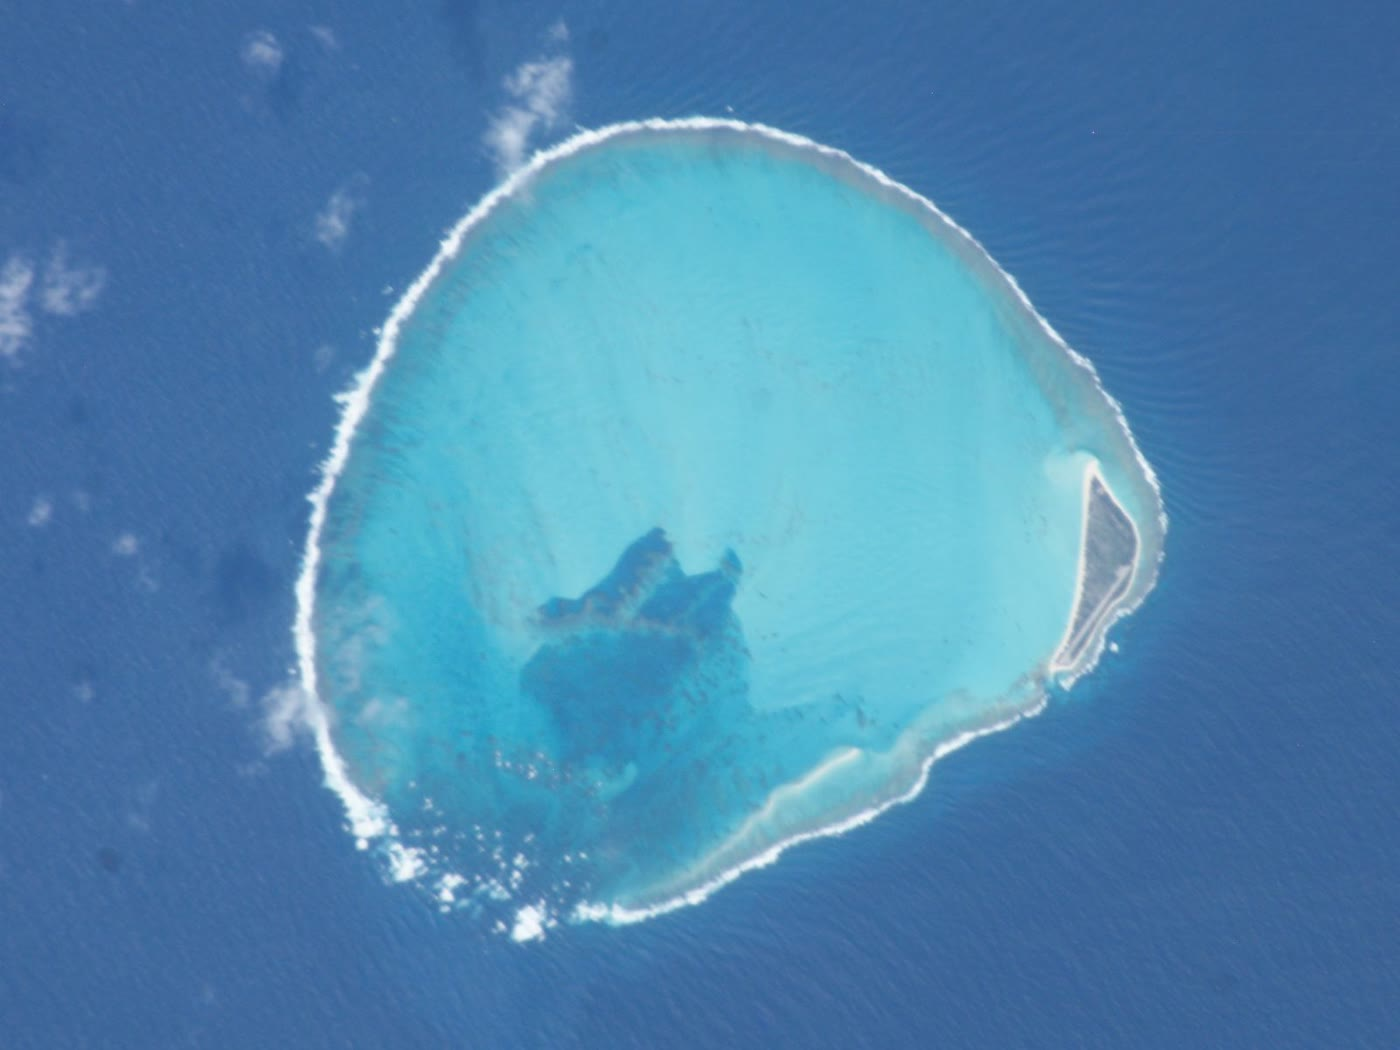
\includegraphics[width=0.52\linewidth]{images/book4/b2-17-kure-atoll.jpg}
\par\smallskip{\small Het \omterm{def:b2:oceanic-islands:reefs}{atol} Kure, het noordelijkste koraalatol, gefotografeerd door een astronaut vanuit
het Internationaal Ruimtestation op 22 februari 2004. De ring van rif, hoogstens ongeveer tien kilometer
breed, omsluit een lagune; het enige permanente eiland, Green Island, ligt op de rand (rechts). NASA,
publiek domein, via Wikimedia Commons.}
\end{omfigure}
% ledger: pmnm:kure (6 miles = 9.7 km)

\section{Erosie, zeeniveau en het einde van een eiland}\label{sec:b2:oceanic-islands:erosion}

Terwijl het zinkt, wordt een eiland ook afgesleten. Een hoog eiland vangt de passaatwinden: op de
loefhellingen van de Hawaïaanse vulkanen valt plaatselijk meer dan \qty{9}{m} regen per jaar.
Beken snijden in minder dan een miljoen jaar diepe canyons uit, zoals op Kohala, op het eiland Hawaï.
Sommige grote kliffen die ooit als het werk van erosie alleen werden gezien, zoals de zeekliffen van het noorden van
Molokai, worden nu gelezen als de achterwanden van reusachtige afschuivingen, die sindsdien zijn teruggeschreden. Golven tasten de kust aan en
schaven er een abrasieplatform op zeeniveau omheen. Erosie en wegzinken samen verwijderen elk spoor
van vulkanisch gesteente boven de zee in ongeveer \qty{15}{Myr}. Gardner Pinnacles, van ongeveer die ouderdom, is
het oudste eiland van de keten waar nog vulkanisch gesteente boven het water uitsteekt. Verder naar het
noordwesten zijn er alleen zandeilanden, \omterm{def:b2:oceanic-islands:reefs}{atollen} en verdronken vulkanen.
% ledger: cs14:erosion, cs14:erase

De zeespiegel staat ondertussen niet stil. Tijdens het laatste glaciale maximum lag hij ongeveer
\qty{120}{m} lager dan vandaag. De kust van een eiland lag toen lager op zijn flanken, en de riffen
die het nu omzomen waren droog land. Toen het ijs smolt, steeg de zee gemiddeld \qty{12}{m}
per duizend jaar tijdens de grote deglaciatie, van 16.5 tot \qty{8.2}{ka}. Tijdens
smeltwaterpuls 1A steeg ze met minstens \qty{40}{mm} per jaar. Een rif op een zinkende vulkaan moet beide
stijgingen volgen. Voor de noordwestkust van het eiland Hawaï vormen minstens zes verdronken riffen een
trap op de flank, het oudste het diepst. Elk groeide aan de kust, raakte achter tijdens een stijging
van de zee, en werd omlaaggevoerd door de belasting van het jonge eiland. Zodra een vulkaan meer dan
ongeveer \qty{125}{m} is gezonken, de amplitude van het glaciale zeeniveau, komt hij niet meer terug in de golven.
% ledger: usgs:lgm (Book 1), lambeck14:lgm (Book 2), cs14:erase, cs14:subsidence

De welving kan de andere kant op werken. Oahu ligt op de bolling die door de last van de jongere eilanden is opgeheven,
en is een beetje gerezen: riffen van het laatste interglaciaal, 133 tot \qty{115}{ka} oud, dagzomen rondom
het eiland, en een rif van ongeveer \qty{334}{ka} oud staat nu \qty{21}{m} boven zeeniveau. Het
einde van een \omterm{def:b2:oceanic-islands:stages}{oceaaneiland} staat dus in zijn gesteenten en zijn riffen geschreven. Lava bouwt het op, afschuivingen en
regen breken het af, golven schaven het af, de plaat voert het omlaag, en een rif houdt zijn plaats aan het
oppervlak tot koud water en een stijgende zee ook dat laten verdrinken.
% ledger: cs14:arch

\section*{Oefeningen}\label{sec:b2:oceanic-islands:exercises}

Gegevens voor de oefeningen, tenzij anders vermeld: diepte--ouderdomswet $d = \qty{2500}{m} + C\sqrt t$ met
$C = \qty{350}{m.Myr^{-1/2}}$ voor $0 \le t \le \qty{70}{Myr}$, en $d = \qty{6400}{m} -
\qty{3200}{m}\,e^{-t/62.8}$ boven \qty{20}{Myr}; $1~\text{voet} = \qty{0.3048}{m}$, $1~\text{vadem}
= \qty{1.8288}{m}$, $1~\text{mijl} = \qty{1.609}{km}$; rifgroei tot \qty{4.2}{mm.yr^{-1}}.

\begin{exercise}[$\star$]\label{exo:b2:oceanic-islands:1}
Benoem het stadium van elke vulkaan: (a) een \omterm{def:b2:oceanic-islands:seamount}{zeeberg} waarvan de top \qty{975}{m} onder de zee ligt en die
alkalische lava uitstoot; (b) een vulkaan boven de hotspot die met hoge snelheid tholeïtische lava uitstoot; (c) een
uitgedoofde vulkaan waarvan de laatste stromen, alkalischer dan het grootste deel van het eiland, het schild afdekken; (d) een
eiland waar, na een stilte van \qty{2}{Myr}, enkele kleine alkalische monden opengaan; (e) een ring van rif
rond een lagune zonder vulkanisch gesteente in zicht.
\end{exercise}

\begin{exercise}[$\star$]\label{exo:b2:oceanic-islands:2}
Een vulkaan wordt gebouwd op een plaat van \qty{9}{Myr} oud. (a) Hoe diep ligt de zeebodem eromheen? (b) Hoe
ver zal hij gezonken zijn wanneer de plaat \qty{25}{Myr} oud is? (c) Met welke snelheid zinkt hij dan?
\end{exercise}

\begin{exercise}[$\star$]\label{exo:b2:oceanic-islands:3}
Zeventien grote afschuivingen vormden zich in de laatste \qty{5}{Myr} rond de Hawaïaanse hoofdeilanden, en
zeventig langs de Hawaïaanse Rug in \qty{30}{Myr}. (a) Bepaal in elk geval het gemiddelde interval tussen twee afschuivingen.
(b) Waarom zijn beide slechts bovengrenzen van het werkelijke interval?
\end{exercise}

\begin{exercise}[$\star$]\label{exo:b2:oceanic-islands:4}
Op Enewetak werd in het ene boorgat basalt aangetroffen op 4158 voet en in het andere harde sokkel op 4610 voet;
de rifkoralen aan de basis van de kalksteen leven niet dieper dan 150 voet. (a) Reken
de drie diepten om naar meter. (b) Met minstens hoeveel is de top van de vulkaan onder Parry Island
gezonken sinds het eerste rif erop groeide? (c) De basis van de kalksteen is Eoceen, dus minstens
\qty{33.9}{Myr} oud. Wat is de grootst mogelijke gemiddelde zinksnelheid?
\end{exercise}

\begin{exercise}[$\star\star$]\label{exo:b2:oceanic-islands:5}
(a) Bepaal de snelheid van thermisch wegzinken, in \unit{m} per \unit{Myr} en in \unit{mm.yr^{-1}}, van
eilanden op platen van 4, 25 en \qty{49}{Myr} oud. (b) Hoeveel keer sneller dan de snelste hiervan
kan een productief rif groeien? (c) En hoeveel keer sneller is de belastingsfase voor het eiland
Hawaï, \qty{2.6}{m} per duizend jaar?
\end{exercise}

\begin{exercise}[$\star\star$]\label{exo:b2:oceanic-islands:6}
(a) Bepaal met de exponentiële wet de zinksnelheid op een plaat van \qty{100}{Myr} oud, in \unit{m}
per duizend jaar, en vergelijk die met de \qty{0.01}{m} per duizend jaar die langs de
Hawaïaanse Rug is gemeten. (b) Bij welke plaatouderdom is de snelheid precies \qty{10}{m.Myr^{-1}}? (c) Ga na dat de
twee wetten bijna dezelfde diepte geven voor een plaat van \qty{25}{Myr} oud.
\end{exercise}

\begin{exercise}[$\star\star$]\label{exo:b2:oceanic-islands:7}
De Hawaïaanse riffen verdrinken ongeveer \qty{33}{Myr} na de geboorte van hun vulkaan, en het vulkanisme verplaatst zich
langs de keten met \qty{8.6}{cm.yr^{-1}}. (a) Hoe ver van de hotspot ligt een eiland wanneer zijn
rif verdrinkt? (b) Midway is een \omterm{def:b2:oceanic-islands:reefs}{atol} van \qty{27.7}{Myr} oud: is het consistent dat het nog een
levend rif heeft? (c) Kure ligt 55 mijl voorbij Midway. Schat zijn ouderdom, en zeg of het dicht
bij het \omterm{def:b2:oceanic-islands:darwin-point}{Darwinpunt} ligt.
\end{exercise}

\begin{exercise}[$\star\star$]\label{exo:b2:oceanic-islands:8}
In de \omterm{def:b2:oceanic-islands:collapse}{Nuuanu-puinlawine} is de \omterm{def:b2:oceanic-islands:seamount}{Tuscaloosa-zeeberg} een blok van ongeveer \qty{30}{km} lang,
\qty{17}{km} breed en minstens \qty{2}{km} hoog. (a) Welk volume zou een doos met deze afmetingen
bevatten? En een piramide op hetzelfde grondvlak en met dezelfde hoogte? (b) Vergelijk met het volume van de
Kilauea, \qty{10000}{km^3}. (c) De lawine bedekt \qty{23000}{km^2}. Als ze gemiddeld
\qty{100}{m} dik was (een aanname: haar dikte ver van Oahu is slecht bekend), wat zou haar
volume dan zijn?
\end{exercise}

\begin{exercise}[$\star\star$]\label{exo:b2:oceanic-islands:9}
Voor het eiland Hawaï zinkt de flank met \qty{2.6}{m} per duizend jaar onder de last van de
vulkaan. (a) Hoe lang duurt het om een kustlijn \qty{1}{km} diep te laten verdrinken? (b) Een rif dat met
\qty{4.2}{mm.yr^{-1}} groeit, ligt op deze flank. Houdt het bij wanneer de zeespiegel constant is? (c) Tijdens de
grote deglaciatie, van 16.5 tot \qty{8.2}{ka}, steeg de zee gemiddeld met \qty{12}{mm.yr^{-1}}. Hoe
diep ligt de top van het rif aan het einde, als het aan het oppervlak begon? (d) Hetzelfde, voor een rif op
een oude vulkaan die niet meer zinkt.
\end{exercise}

\begin{exercise}[$\star\star\star$]\label{exo:b2:oceanic-islands:10}
(a) Toon aan dat, over een vast interval $\Delta$, de wortelwet een eiland minder laat zinken naarmate zijn
plaat ouder is. (b) Bereken het wegzinken over \qty{20}{Myr} voor een eiland dat op de rug is geboren en voor een eiland dat
op een plaat van \qty{50}{Myr} oud is geboren. (c) De plaat onder een rug is zeer heet, en de wortelwet geeft een
oneindige snelheid bij $t = 0$. Is dat een probleem voor het wegzinken over een eindig interval? Leg uit.
\end{exercise}

\begin{exercise}[$\star\star\star$]\label{exo:b2:oceanic-islands:11}
Een \omterm{def:b2:oceanic-islands:reefs}{atol} zinkt met \qty{30}{m.Myr^{-1}}, en de zeespiegel schommelt met de ijstijden met ongeveer \qty{120}{m},
in cycli van ongeveer \qty{100}{kyr}. (a) Hoe ver zinkt het \omterm{def:b2:oceanic-islands:reefs}{atol} tijdens één cyclus? (b) Hoe hoog
staat de top van het \omterm{def:b2:oceanic-islands:reefs}{atol} bij een glaciale laagstand boven de zee? Wat gebeurt er dan met het
rifgesteente? (c) Hoeveel cycli zijn er nodig voordat het \omterm{def:b2:oceanic-islands:reefs}{atol} de volle \qty{120}{m} is gezonken?
(d) Verklaar de uitgeloogde zones die in de boorgaten van Enewetak zijn gevonden, en waarom
\cref{prop:b2:oceanic-islands:cap} op lange termijn toch de dikte van de kap geeft.
\end{exercise}

\begin{exercise}[$\star\star\star$]\label{exo:b2:oceanic-islands:12}
Een \omterm{def:b2:oceanic-islands:reefs}{atol} verdrinkt wanneer zijn plaat \qty{50}{Myr} oud is: zijn rif raakt achter en zijn top eindigt op de
groeigrens van de diepste kalkalgen, \qty{150}{m} onder de zee. (a) Hoeveel zinkt het met de exponentiële
wet nog verder voordat de plaat \qty{120}{Myr} oud is? (b) Hoe diep ligt de top
van de \omterm{def:b2:oceanic-islands:seamount}{guyot} dan? (c) Een \omterm{def:b2:oceanic-islands:seamount}{guyot} naast Enewetak heeft zijn top op 700 vadem. Reken om, en vergelijk.
(d) Noem twee redenen waarom een echte \omterm{def:b2:oceanic-islands:seamount}{guyot} dieper of ondieper kan liggen dan deze schatting.
\end{exercise}

\begin{problem}[{Weekendprobleem --- Van vulkaan tot atol}]\label{pb:b2:oceanic-islands:1}
Het verzonnen eiland Petrel wordt geboren boven een hotspot op een plaat van \qty{10}{Myr} oud. Zijn vulkaan is
een kegel met een basisstraal van \qty{50}{km}. Wanneer zijn groei eindigt, staat zijn top \qty{1000}{m} boven
zeeniveau. Zijn laatste vulkanische gesteente verdwijnt \qty{12}{Myr} later onder zeeniveau. Een rif houdt
dan zijn top op zeeniveau tot de plaat \qty{70}{Myr} oud is, wanneer het \omterm{def:b2:oceanic-islands:reefs}{atol} het
\omterm{def:b2:oceanic-islands:darwin-point}{Darwinpunt} passeert. Gebruik de diepte--ouderdomswet van de oefeningen (de wortelwet tot \qty{70}{Myr}, de
exponentiële wet daarboven), een rifgroei van \qty{4.2}{mm.yr^{-1}} en de gegevens van het hoofdstuk.
De zeespiegel wordt constant genomen, behalve in de vragen 8 tot 10. Rond diepten af op de meter.

\noindent\textbf{Deel I --- Groei.}
\begin{enumerate}
  \item Hoe diep ligt de zeebodem waar Petrel wordt geboren?
  \item Wat is de hoogte van de vulkaan boven die bodem wanneer zijn groei eindigt, als men het
        wegzinken van de bodem onder de last verwaarloost?
  \item Bepaal het volume van de kegel.
  \item Als \qty{85}{\percent} ervan werd uitgestoten tijdens een \omterm{def:b2:oceanic-islands:stages}{schildstadium} van \qty{1}{Myr}, wat was dan de
        gemiddelde eruptiesnelheid? Vergelijk met de toevoer van de Kilauea vandaag, ongeveer
        \qty{0.1}{km^3} per jaar.
  \item Hoeveel Petrels zouden één Mauna Loa vormen, met \qty{95600}{km^3}?
  \item Welke lava's, tholeïtische of alkalische, vormen het grootste deel van de kegel? Welke dekken hem af?
\end{enumerate}

\noindent\textbf{Deel II --- Belasting en verdronken riffen.}
\begin{enumerate}[resume]
  \item Tijdens zijn groei laat de last het jonge eiland \qty{1}{km} zinken in \qty{1}{Myr}. Wat is
        de gemiddelde snelheid, en hoe verhoudt die zich tot de \qty{2.6}{m} per duizend jaar die
        voor het eiland Hawaï is gemeten?
  \item Een rif groeit tijdens deze fase aan de kust, bij een constante zeespiegel. Houdt het bij, en
        met welke marge?
  \item De zeespiegel stijgt daarna met \qty{12}{mm.yr^{-1}}. Hoeveel raakt het rif elk jaar
        achter?
  \item Hoe lang duurt het voordat zijn top \qty{150}{m} bereikt, de diepste groeigrens? Wat laat dat
        achter op de flank van het eiland?
\end{enumerate}

\noindent\textbf{Deel III --- Wegzinken en erosie.}
\begin{enumerate}[resume]
  \item Hoeveel is Petrel gezonken tegen de tijd dat zijn laatste vulkanische gesteente verdwijnt, als de plaat
        dan \qty{22}{Myr} oud is?
  \item Hoeveel van de \qty{1000}{m} van de top heeft erosie weggenomen, en met welke gemiddelde snelheid?
  \item Met welke snelheid zinkt Petrel wanneer zijn groei eindigt, en wanneer zijn top verdwijnt?
  \item Hoe diep ligt de zeebodem eromheen op dat moment?
  \item Vergelijk de \qty{12}{Myr} die het duurde met de \qty{15}{Myr} van de Hawaï-eilanden. Geef een
        reden waarom een hoog Hawaïaans eiland langer standhoudt.
  \item Noem twee processen, naast regen en rivieren, die het eiland boven zeeniveau wegnemen.
  \item Welke vorm van rif omringt Petrel kort voordat zijn top verdwijnt?
\end{enumerate}

\noindent\textbf{Deel IV --- Atol en guyot.}
\begin{enumerate}[resume]
  \item Hoe dik is de rifkap wanneer de plaat \qty{70}{Myr} oud is?
  \item Welke gemiddelde rifgroei was daarvoor nodig? Hoeveel keer kleiner is die dan de groei
        die het rif kon halen?
  \item Vergelijk de kap met de diepte van het basalt onder Enewetak.
  \item Hoe diep ligt de zeebodem rond het \omterm{def:b2:oceanic-islands:reefs}{atol} wanneer het het \omterm{def:b2:oceanic-islands:darwin-point}{Darwinpunt} passeert?
  \item Hoeveel zinkt het verdronken \omterm{def:b2:oceanic-islands:reefs}{atol} met de exponentiële wet nog verder voordat de plaat
        \qty{120}{Myr} oud is?
  \item Als de top van het rif bij het verdrinken op \qty{150}{m} stopte, hoe diep ligt de top van de
        \omterm{def:b2:oceanic-islands:seamount}{guyot} dan?
  \item Samengevat: hoe dik is de rifkap van het \omterm{def:b2:oceanic-islands:reefs}{atol} Petrel?
\end{enumerate}
\end{problem}
